\section{Methods} \label{sec:methods}

include figure with example subsampled phylogenies

describe why we allow true polytomies to be resolved either way by reconstructions: because in treatments where there is no MRCA (two or more original lineages exist) you have a big polytomy at the root and most sampled triplets go through this big polytomy.
So when we measure triplet distance, we won't count resolving a true polytomy into two nodes as an error.
We include strict triplet distance in the supplement.

If it is critical to differentiate lineages with different founders, you can easily add a unique fixed heritable tag to each founder.

\begin{figure}
  \centering
  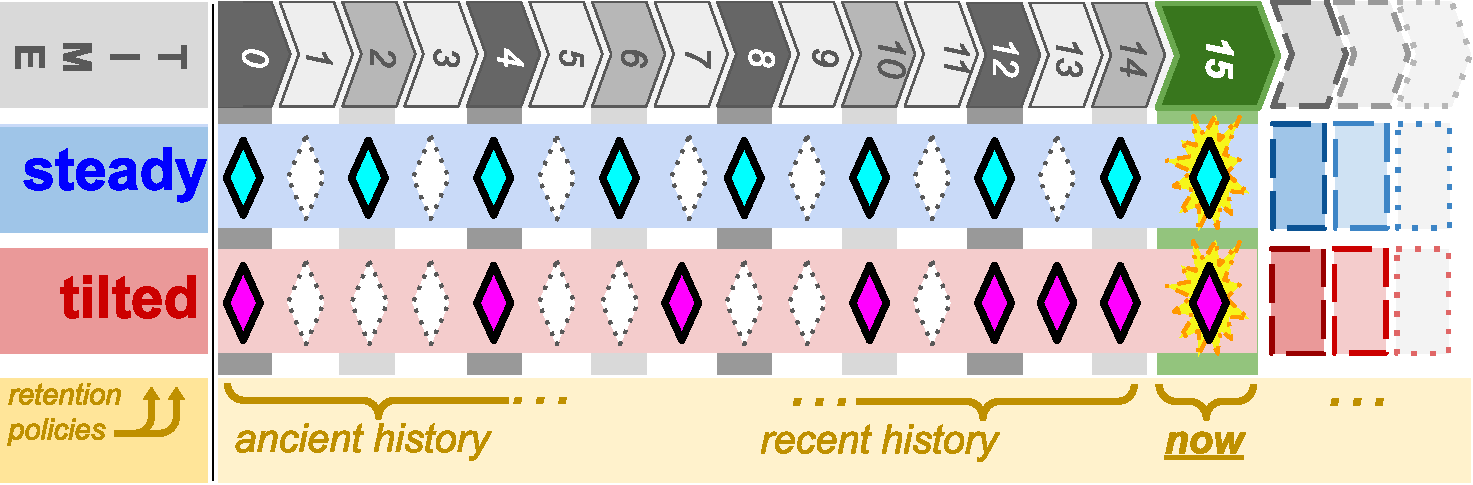
\includegraphics[width=\linewidth]{img/steady-vs-tilted-schematic}
  \caption{%
  \textbf{Steady versus tilted retention policy.}
  Steady policy (top) retains differentia with time points spaced evenly across history.
  Tilted policy (bottom) retains differentia more densely over recent history, giving gap size proportional to time ago.
  Hybrid policy (not shown) allocates half of available space to hold tilted data and half to hold steady.
  }
  \label{fig:steady-vs-tilted-schematic}
\end{figure}

